\section{Remote Interface}
\label{cha:Remote}
\subsection{ General Information}

\textbf{Two remote interfaces are standard in the instrument:}

\begin{itemize}
\item A simple ground closure parallel interface, which allows remote control of some of the major operational parameters of the PT 5300
\item A serial remote gives control over all the functions of the PT 5300. The serial remoteoperates by use of an RS 232 communication port. 
\end{itemize}

To select type of remote interface move cable between connectors PAR (XM1) and SER (XR1) on Main Board (Unit 1).

\begin{figure}[hbt]
\centering
\includegraphics[width=0.5\textwidth]{fig/pt5300_overview}
\caption{Location of Connectors}
\end{figure}

\subsection{Parallel Remote}

The following parameters can be controlled when the remote connector is configured for parallel
ground closure control:
\begin{itemize}
\item Recall of preset \#1 to \#8
\item Selection of genlock mode
\end{itemize}

\subsubsection{Connector Description}

\textbf{Connector type:}
9 pin sub-D

\begin{figure}[hbt]
\centering
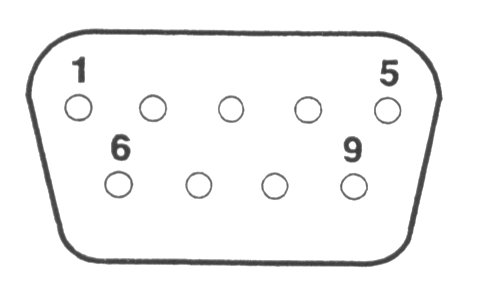
\includegraphics[width=0.5\textwidth]{fig/dsub}
\caption{Remote connector seen from rear panel}
\end{figure}

\begin{tabular*}{\textwidth}{@{\extracolsep{\fill}}|l|p{28em}|}
\hline
\textbf{Pin no.:} & \textbf{Function:} \\ \hline
1 & Preset 0 (LSB) \\ \hline
2 & Preset 1 \\ \hline
3 & Preset 2 (MSB) \\ \hline
4 & Genlock/Preset selection: \\
  & 0: Selects pin 6 active (pin 1-3 inactive) - genlock. \\ 
  & 1: Selects pin 1-3 active (pin 6 inactive) - preset. \\ \hline
5 & Ground \\ \hline
6 & Genlock selection: \\
  & 0: Selects external genlock (the result is unlocked if no valid signal is found in the active input). \\
  & 1: Selects internal reference. \\ \hline
7 & Genlock status output: \\
  & 0: Unlocked (using internal reference) \\
  & 1: Gen-locked or internal. \\ \hline
8 & Warning output: \\
  & 0: Error detected internal in the generator. \\
  & 1: No errors. \\ \hline
9 & Remote enable: \\
  & 0: Remote enabled. \\
  & 1: Remote disabled. \\ \hline
\end{tabular*}

\textbf{Note:} All outputs have internal pull up resistors to +5 V.

\textbf{Note:} The Presets are numbered binary. The binary number is one less than the number used in the menu system on the front of the generator.

\textbf{Note:} The remote output pins 7 and 8 are active even when the remote is disabled. The remote only has to be configured as parallel.

\textbf{Table of the selections:}

{\tiny
\begin{tabular}{|l|l|l|l|l|l|l|l|l|l|l|}
\hline
\textbf{Function:}		& \textbf{Pin 3} & \textbf{Pin 2} & \textbf{Pin 1} & \textbf{Pin 4} & \textbf{Pin 5} & \textbf{Pin 6} & \textbf{Pin 7} & \textbf{Pin 8} & \textbf{Pin 9} \\ \hline
 & \textbf{(MSB)} & \textbf{(LSB)} & & & & & & & \\ \hline
\textbf{Remote disabled} 	& X & X & X & X & GND & X & OUT & OUT & 1 \\ \hline
\textbf{Preset 1}					& 0 & 0 & 0 & 1 & GND & X & OUT & OUT & 0 \\ \hline
\textbf{Preset 2} 				& 0 & 0 & 1 & 1 & GND & X & OUT & OUT & 0 \\ \hline
\textbf{Preset 3}					& 0 & 1 & 0 & 1 & GND & X & OUT & OUT & 0 \\ \hline
\textbf{Preset 4}					& 0 & 1 & 1 & 1 & GND & X & OUT & OUT & 0 \\ \hline
\textbf{Preset 5}					& 1 & 0 & 0 & 1 & GND & X & OUT & OUT & 0 \\ \hline
\textbf{Preset 6}					& 1 & 0 & 1 & 1 & GND & X & OUT & OUT & 0 \\ \hline
\textbf{Preset 7}					& 1 & 1 & 0 & 1 & GND & X & OUT & OUT & 0 \\ \hline
\textbf{Preset 8}					& 1 & 1 & 1 & 1 & GND & X & OUT & OUT & 0 \\ \hline
\textbf{Genlock Int.}	& X & X & X & 0 & GND & 1 & OUT & OUT & 0 \\ \hline
\textbf{Genlock Ext.}	& X & X & X & 0 & GND & 0 & OUT & OUT & 0 \\ \hline
\end{tabular}
}

\subsection{Serial Remote}

The serial remote allows for control of virtually all functions in the generator as well as reading of instrument setting.
The serial remote operates electrically as an RS 232C communication port. %The parameter setting for the RS 232 communication port is described in xxx

\begin{figure}[hbt]
\centering
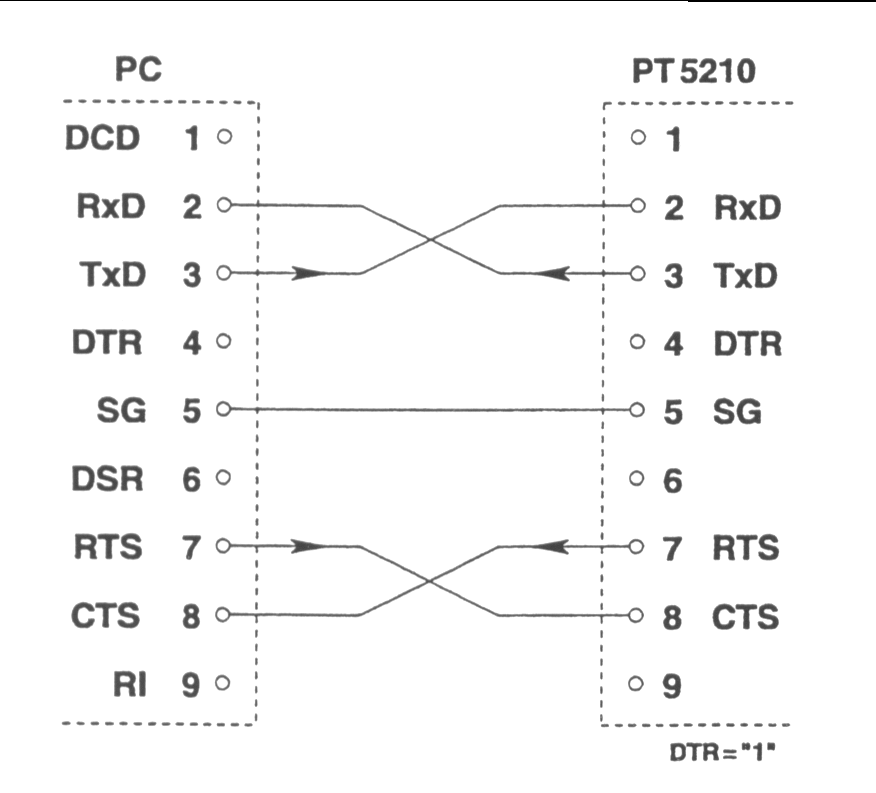
\includegraphics[width=0.5\textwidth]{fig/RS232_connection}
\caption{Configuration of cable between PC and PT 5300}
\end{figure}

The PT 5300 communication protocol complies with the:
\begin{itemize}
\item SCPI 1995.0: Standard Commands for Programmable Instruments, Vol I-IV. This protocol which is based on the IEEE 488.2 (IEEE Standard Codes, Formats, Protocols, and Common Commands). 
\end{itemize}

For the description of the commands a basic knowledge of operation of the instrument is assumed.

To use the serial remote a basic knowledge of the SCPI programming and computer control is also recommended. The paper: ``A beginner's Guide to SCPI'' by Barry Epler, Hewlett-Packard Press \copyright, 1991 can be used to gain the basic knowledge of the ideas behind the SCPI system.

\subsection{General Description of the Interface Syntax}

\subsubsection{General Information}
The remote system is organised in a tree structure. The structure defines sub-systems. In order to access command lower in the tree or in different branches the entire command string should be used. Indentation is used to indicate the root level and the branches. The highest level to the left. The complete command always includes all the root levels.

A space between a command string and an option is required, except in a query * where a space is not allowed.

Enter more than one command on a line by using a semicolon ``;'' as divider. A command line is terminated by $<$CR$> <$LF$>$. If the next command is part of the same command system the separation is a ``;'' only. If the next command is part of another command system the ``;'' is followed by a ``;''.

Parameters are separated from the header by a space. Several parameters are separated by a comma. 

Character strings should be placed in single or double quotation marks. 

The valid parameter ranges are shown in the command tables. Non valid values generate an error message.

\subsubsection{Syntax Elements}

\begin{tabular*}{\textwidth}{@{\extracolsep{\fill}}|l|p{28em}|}
; 		& Semicolon separates two commands of a command line and does not change the path.\\
: 		& Colon separates the keywords of a command. In a command line, a colon ``:'' after a separating semicolon ``;'' indicates the root control level.\\
, 		& Comma separates the parameter command.\\
? 		& Question mark identifies a query command (Query commands are formed by adding a question mark to the header).\\
* 		& Asterisk identifies a common command. (Common commands consists of a header preceded by an asterisk and possibly followed by one or more parameters)\\
' or '' & Single or double quote introduces and terminates a character string.\\
\# 		& Double dagger introduces block data. \\
Space & Space Character separates header and parameters.\\
$|$		& Parameters divided by a ``$|$'' indicates an ``or'' selection between the values shown. Only one value may be used at a time.\\
$[$xxxx$]$ & Square brackets indicate an optional specific string parameter used by some command systems.\\
XXXX 	& A vertical line through a command indicates a command not implemented. The command is included for future compatibility
reasons. The generator will not give any response to these command (error messages are not generated).\\
\end{tabular*}

\subsubsection{Command Syntax}

A command consists of a ``header'' and one or several ``parameters''. Header and parameters are separated by space. A header may consist of several keywords.

\subsubsection{Syntax of Program Messages}

A command or query is called a program message unit. Such a program message unit consists of a header, or a header separated by a space from one or more parameters. The program header separator between the header and the first parameter must be at least one ``whitespace'' character. The header consists of one or more mnemonics (key words) describing the command. The parameters in a message unit are also referred to as ``Data Elements''. They are mutually separated by a comma (,), which is referred to as ``Data Separator''. Furthermore the following rules are valid:

\begin{itemize}
\item Any one of the ``white space'' characters (dec. 0..9, 11.. 32) may:
\begin{itemize}
\item Precede a header
\item Precede the Message Terminator
\item Be placed in between the header and the parameter
\item Be placed in between two consecutive parameters
\item String data in a parameter must be specified between quotes. A quote may either be a
\end{itemize}
\item `single quote' (dec. 39) or a ``double quote'' character (dec. 34)
\end{itemize}

One or more program message units (commands) may be send within a single program message. Program message units are separated by a semicolon (;). A message of one or more units is terminated by a program message terminator.

The program message terminator must be the following code:
\begin{itemize}
\item LF <line feed> (dec.10) code
\end{itemize}

\textbf{Note:} Most controller programming languages send the terminator automatically, but allow it to be changed.

\textbf{Basically there are two types of program headers:}
\begin{itemize}
\item Compound headers - Commands have a compound header consisting of one of more key words (mnemonics), mutually separated by a colon (:) character. Such as a colon may also precede the header.
\item Command headers - The program messages that are standardised are called common commands. Their headers always start with an asterisk (*) character 
\end{itemize}

Each key word in a compound command header represents a node in the command tree. The left most key word is the root node, representing the highest hierarchical level in the command tree. Subsequent keyword represents sub nodes under the root node.

\subsubsection{Long and Short Form}

Program messages may be sent in either long or short form
\begin{itemize}
\item The long form is the full word
\item The short form is the first character of the long form
\end{itemize}

The short form in a syntax specification is shown in upper case, and the remaining part of the long form is shown in lower case characters.

\textbf{Note:} Upper and lower case, as used in syntax specification, is only a notation habit to facilitate distinction between long and short form. The generator itself does not differentiate between upper and lower case characters. In program messages, either the long or short form may be used in any mix of upper or lower case characters. There is no semantic difference between upper and lower case in program messages.

\subsubsection{Syntax of Response Messages}
The response to a query is a response message unit, consisting of one or more parameters (data elements). Successive parameters are separated by a comma (,). If there are multiple queries in a program message, the multiple response message units are grouped together in the corresponding response message. 

Response message units are separated by a semicolon (;) and are terminated by a response message terminator. 

The instrument will always send the response data in short form and in capitals. Headers are not sent in the response messages, parameters only.

